\documentclass[tikz, margin=3mm]{standalone}
\usetikzlibrary{matrix}
\newcommand\x{\times}

\begin{document}
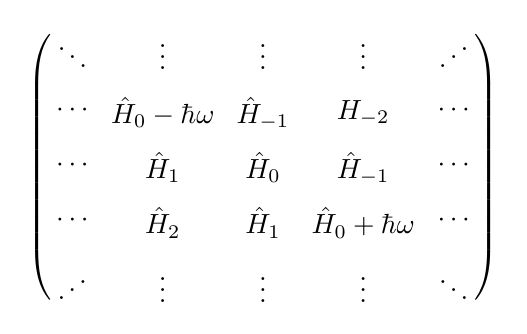
\begin{tikzpicture}
  \matrix [matrix of math nodes,
           nodes={rectangle, %draw, very thin,
                  minimum size=1.2em, text depth=0.25ex,
                  inner sep=0pt, outer sep=0pt,
                  fill opacity=0.5, text opacity=1,
                  anchor=center},
           column sep=20.\pgflinewidth,
           row sep=20.\pgflinewidth,
           inner sep=0pt,
           left delimiter=(,
           right delimiter=),
           ]
  {
    \ddots & \vdots & \vdots & \vdots & \reflectbox{$\ddots$} \\
    \cdots & \hat H_0 - \hbar \omega  & \hat H_{-1} & H_{-2} & \cdots \\
    \cdots & \hat H_{1}  & \hat H_0 & \hat H_{-1} & \cdots \\
    \cdots & \hat H_{2}  & \hat H_1 & \hat H_{0} + \hbar \omega & \cdots \\
    \reflectbox{$\ddots$} & \vdots & \vdots & \vdots & \ddots \\
  };
\end{tikzpicture}

\end{document}
